\documentclass[tikz,border=0pt]{standalone}
\usepackage{amsmath}
\usepackage[scaled]{helvet}
\renewcommand{\familydefault}{\sfdefault}
\usetikzlibrary{arrows.meta,calc,positioning}
\definecolor{navy}{HTML}{101828}
\definecolor{surface}{HTML}{172033}
\definecolor{blue}{HTML}{3987E5}
\definecolor{orange}{HTML}{D95926}
\definecolor{aqua}{HTML}{199E70}
\definecolor{mist}{HTML}{EAF2FB}
\definecolor{muted}{HTML}{98A2B3}
\newcommand{\bitrow}[6]{%
  \node[anchor=east,text=muted,font=\small] at (2.15,#2) {$i=#1$};
  \foreach \b [count=\k from 0] in {#3,#4,#5,#6} {
    \pgfmathsetmacro{\x}{2.55 + .72*\k}
    \fill[blue!18,rounded corners=2pt] (\x,#2-.28) rectangle +(0.58,.56);
    \draw[blue!70,line width=.6pt,rounded corners=2pt] (\x,#2-.28) rectangle +(0.58,.56);
    \node[text=mist,font=\ttfamily\small] at (\x+.29,#2) {\b};
  }
}
\begin{document}
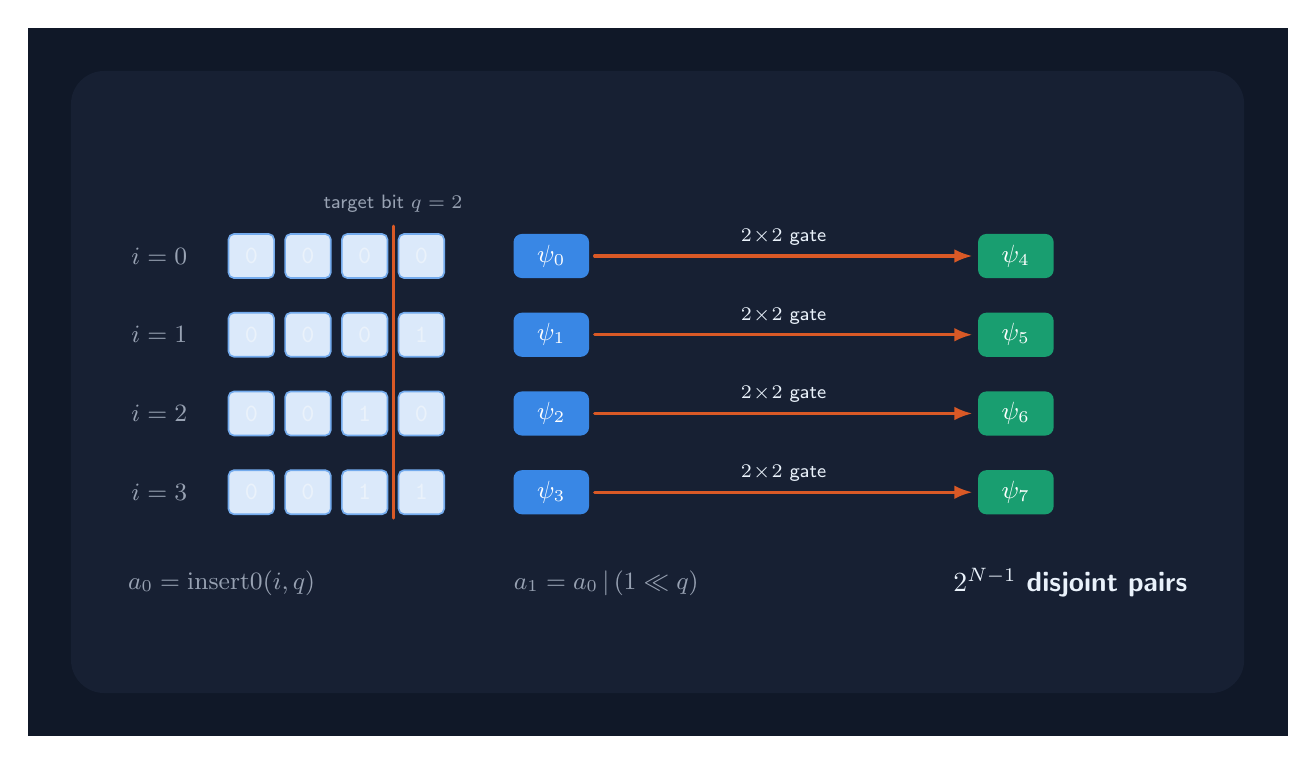
\begin{tikzpicture}[x=1cm,y=1cm,line cap=round,line join=round,font=\sffamily]
  \path[use as bounding box] (0,0) rectangle (16,9);
  \fill[navy] (0,0) rectangle (16,9);
  \fill[surface,rounded corners=12pt] (.55,.55) rectangle (15.45,8.45);

  \begin{scope}[yshift=0.35cm]
  \bitrow{0}{5.75}{0}{0}{0}{0}
  \bitrow{1}{4.75}{0}{0}{0}{1}
  \bitrow{2}{3.75}{0}{0}{1}{0}
  \bitrow{3}{2.75}{0}{0}{1}{1}

  \node[text=muted,font=\scriptsize] at (4.64,6.42) {target bit $q=2$};
  \draw[orange,line width=1.1pt] (4.64,6.13) -- (4.64,2.42);

  \foreach \lo/\hi/\y in {0/4/5.75,1/5/4.75,2/6/3.75,3/7/2.75}{
    \coordinate (L\lo) at (6.65,\y);
    \coordinate (R\lo) at (12.55,\y);
    \fill[blue,rounded corners=3pt] ($(L\lo)+(-.48,-.28)$) rectangle +(0.96,.56);
    \node[text=white,font=\ttfamily\small] at (L\lo) {$\psi_{\lo}$};
    \fill[aqua,rounded corners=3pt] ($(R\lo)+(-.48,-.28)$) rectangle +(0.96,.56);
    \node[text=white,font=\ttfamily\small] at (R\lo) {$\psi_{\hi}$};
    \draw[-{Latex[length=2.3mm]},orange,line width=1.15pt] ($(L\lo)+(.55,0)$) -- node[above,text=mist,font=\scriptsize] {$2\!\times\!2$ gate} ($(R\lo)+(-.55,0)$);
  }
  \end{scope}

  \node[anchor=west,text=muted,font=\small] at (1.15,1.95) {$a_0=\operatorname{insert0}(i,q)$};
  \node[anchor=west,text=muted,font=\small] at (6.05,1.95) {$a_1=a_0\,\vert\,(1\ll q)$};
  \node[anchor=east,text=mist,font=\bfseries] at (14.85,1.95) {$2^{N-1}$ disjoint pairs};
\end{tikzpicture}
\end{document}
